\guidepart{slate}{Extras}{The extras}
  {The cheat sheet, the command line, and words you might trip over.}
  {\partitem{\iKeyboard}{Keyboard cheat sheet}
   \partitem{\iTerminal}{Command-line options}
   \partitem{\iBrain}{Glossary}}

% =========================================================================================
\chapter{Keyboard cheat sheet}\label{app:keys}
\chapmeta{print it}{Stick this page next to your monitor}

\newcommand\shortcut[2]{#1 & #2\\}
\newcommand\sheet[3]{%
  \begin{tcolorbox}[enhanced, arc=8pt, boxrule=0pt, colback=#1!7, left=10pt, right=10pt, top=8pt, bottom=8pt,
    before skip=0pt, after skip=10pt, fontupper=\small]
  {\heavy\large\color{#1!85!black}#2}\par\vspace{4pt}
  \renewcommand\arraystretch{1.5}\begin{tabularx}{\linewidth}{@{}X>{\raggedleft\arraybackslash}p{36mm}@{}}#3\end{tabularx}
  \end{tcolorbox}}

\begin{multicols}{2}
\sheet{accent}{\iRocket\enspace Everywhere}{%
  \shortcut{Command palette}{\keys{\mod+K}}
  \shortcut{New connection}{\keys{\mod+N}}
  \shortcut{Quick Connect}{\keys{\mod+Shift+Q}}
  \shortcut{Settings}{\keys{\mod+,}}
  \shortcut{Full screen}{\kbd{F11}}}

\sheet{violet}{\iSplit\enspace Tabs \& panes}{%
  \shortcut{Close tab}{\keys{\mod+W}}
  \shortcut{Next tab}{\keys{\mod+Tab}}
  \shortcut{Previous tab}{\keys{\mod+Shift+Tab}}
  \shortcut{Go to tab 1–9}{\keys{\mod+1}…\kbd{9}}
  \shortcut{Split right}{\keys{\mod+Shift+D}}
  \shortcut{Split down}{\keys{\mod+Shift+E}}}

\sheet{teal}{\iWand\enspace Power tools}{%
  \shortcut{Broadcast on/off}{\keys{\mod+Shift+B}}
  \shortcut{Snippets}{\keys{\mod+Shift+S}}
  \shortcut{Record on/off}{\keys{\mod+Shift+R}}}

\sheet{amber}{\iTerminal\enspace In the terminal}{%
  \shortcut{Copy selection}{\keys{\mod+C}}
  \shortcut{Paste}{\keys{\mod+V}}
  \shortcut{Find}{\keys{\mod+F}}
  \shortcut{Next / previous match}{\kbd{Enter} / \keys{Shift+Enter}}
  \shortcut{Scroll a page}{\keys{Shift+PageUp}}
  \shortcut{Top / bottom}{\keys{Shift+Home} / \kbd{End}}
  \shortcut{Previous / next prompt}{\keys{\mod+Shift+Up} / \kbd{Down}}
  \shortcut{Open link}{\kbd{Ctrl}/\kbd{\ph{E1C4}} + click}}

\sheet{pink}{\iMap\enspace Mouse moves}{%
  \shortcut{Select word / line}{double / triple-click}
  \shortcut{Extend selection}{\kbd{Shift} + click}
  \shortcut{Select several profiles}{\kbd{Ctrl}/\kbd{\ph{E1C4}} + click}
  \shortcut{Everything else}{right-click it}}
\end{multicols}

% =========================================================================================
\chapter{Command-line options}\label{app:cli}
\chapmeta{1 minute}{You'll script, demo and test with a few handy flags}

\renewcommand\arraystretch{1.5}
\begin{tabularx}{\linewidth}{@{}>{\leavevmode\ttfamily\color{ink}}p{52mm}X@{}}
  \toprule
  --data-dir DIR        & Use another data folder (portable installs, demos, testing).\\
  --theme pro|midnight|light & Start with this theme.\\
  --connect NAME        & Connect to a saved profile by name at startup. Repeat it for several.\\
  --open WINDOW         & Open a window at startup: \code{settings}, \code{settings:security},
                          \code{settings:diagnostics}, \code{snippets}, \code{keys}, \code{recordings}, \code{palette},
                          \code{quick}…\\
  --run-local CMD       & Open a local shell and run a command in it.\\
  RUST\_LOG=debug        & (environment) More detail in \code{nexus.log}, and on the terminal you started from.\\
  --version             & Print the version and exit.\\
  \bottomrule
\end{tabularx}

\begin{sidequest}[How the screenshots in this guide were made]
Every screenshot here is the real app, driven by \code{docs/guide/tools/screenshots.sh}: it starts throwaway
SSH, IRC, VNC and GitHub-ish servers, fills a demo data folder, and runs Nexus Terminal headless with
\code{--screenshot}, \code{--do} (run a palette command) and \code{--answer} (fill a password prompt; only accepted together with \code{--screenshot}). Change the app,
rerun the script, rebuild the guide.
\end{sidequest}

% =========================================================================================
\chapter{Glossary}\label{app:glossary}
\chapmeta{dip in}{Words you might trip over, in one line each}

\begin{multicols}{2}\small
\begin{description}[leftmargin=0pt, itemsep=5pt]
  \item[Agent] A background program holding your unlocked SSH keys, so you type the passphrase once.
  \item[Asciicast] The file format for terminal recordings. Plays in Nexus Terminal and \code{asciinema}.
  \item[Bastion / jump host] A server you go \emph{through} to reach the ones behind it.
  \item[Baud rate] How fast a serial line talks. Both ends must agree.
  \item[Broadcast] Typing into several sessions at once.
  \item[Certificate authority] A key that vouches for other keys, so servers signed by it are trusted without a prompt.
  \item[DTR / RTS] Serial control lines. Some boards use them for reset or flashing.
  \item[Fingerprint] A short summary of a server's host key, used to spot imposters.
  \item[Host key] A server's identity. Changes when it's rebuilt, or when someone's pretending.
  \item[Keychain] Your operating system's password store.
  \item[NLA] Network Level Authentication: Windows checks your password before building a desktop.
  \item[OSC 133] The escape codes a shell uses to mark its prompts, which powers shell integration.
  \item[Port forward] A tunnel carrying one TCP port through SSH.
  \item[Profile] A saved connection.
  \item[RAW TCP] A plain socket: bytes in, bytes out, no terminal rules.
  \item[RDP] Microsoft's Remote Desktop Protocol, for Windows (and xrdp) desktops.
  \item[SASL] How IRC networks log you in while you connect, instead of messaging NickServ afterwards.
  \item[SFTP] File transfer over SSH.
  \item[Snippet] A saved command, optionally with blanks to fill in.
  \item[TOTP] Time-based one-time passwords: the six digits from your authenticator app.
  \item[Trigger] A rule that watches output and reacts to a pattern.
  \item[Vault] Nexus Terminal's encrypted password store, for when there's no keychain.
  \item[VNC] A way of seeing and controlling another computer's desktop.
\end{description}
\end{multicols}

\vfill
\begin{center}
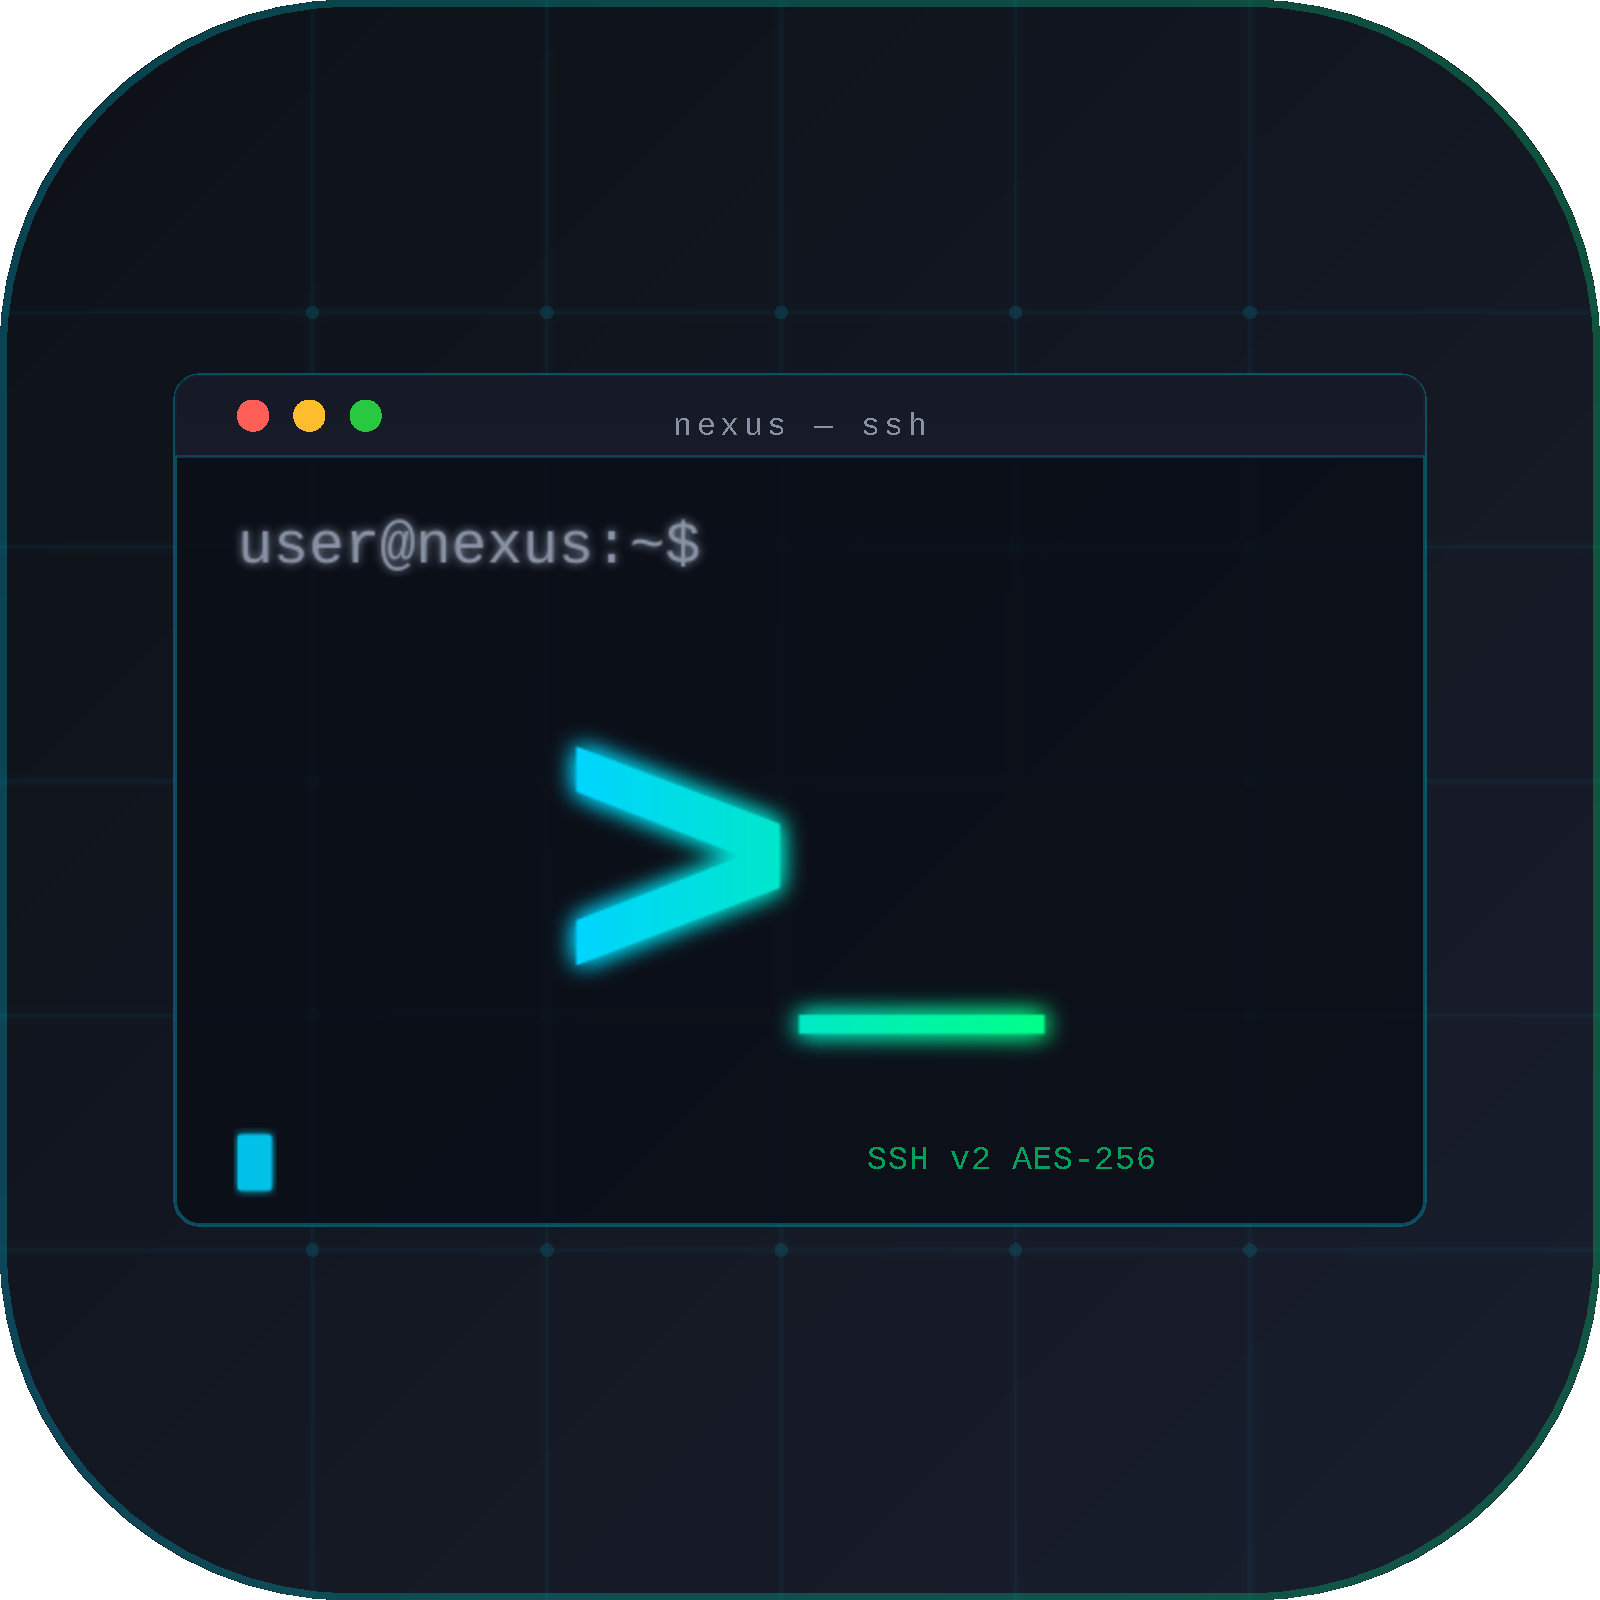
\includegraphics[width=16mm]{img/logo.pdf}\par\vspace{6pt}
{\heavy\color{ink}That's the lot.}\par
{\small\color{muted}Go and connect to something. \iRocket}
\end{center}
